\chapter{Implementierung}\label{chapter:Implementierung}

\section{ObjLoader}
Die ObjLoader-Klasse ist dafür zuständig die Daten aus der Obj-Datei des Modells einzulesen und in das passende Format für OpenGL umzuwandeln.\\
Bei ihrer Instanziierung wird der Klasse der Pfad zu der Datei die eingelesen werden soll übergeben.
Nachdem diese geladen wurde, muss die Datei Zeile für Zeile durchlaufen werden und anhand der Abkürzungen, mit denen jede Zeile beginnt, der Datentyp bestimmt werden. \\
Der Aufbau einer Obj-Datei unterliegt dabei dem folgenden Muster (vergleiche dazu auch Abbildung \ref{fig:obj-datei}):\\
Jede Zeile enthält ein Datenobjekt, welches über die die Kennung zu einem bestimmten Datentyp zugeordnet werden kann. 
Zu Beginn der Datei werden alle Einzelteile des Modells definiert:
\begin{description}
\item[Vertex (v):] Ein Vertex repräsentiert einen Eckpunkt des Objektes. Dazu werden in der Zeile die drei Koordinaten des Punktes gespeichert.
\item[Textur (vt):] Diese Zeile besteht aus zwei Koordinaten, welche einen Punkt in einem zweidimensionalen Bild, der Texturdatei, repräsentieren.
\item[Normalenvektor (vn):] Dieser Kennung folgenden die drei Koordinaten eines Normalenvektors  
\end{description}

\begin{figure}
\centering
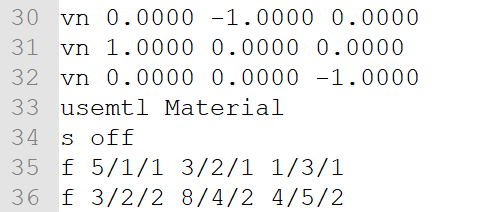
\includegraphics[width=0.8\textwidth]{Abbildungen/obj-datei.png}
\caption[Obj-Dateiformat]{Ausschnitt aus einer Obj-Datei. (Quelle: Eigene Darstellung)}
\label{fig:obj-datei}
\end{figure}
Damit OpenGL mit diesen Einzelteilen arebiten kann, müssen diese noch zusammengesetzt werden. \\
Die dafür nötigen Informationen speichern die sogenannten Faces (deutsch: \glqq Gesichter\grqq ), welche die Kennung f besitzen. Sie beschreiben die einzelnen Flächen des Modells. Da zuvor im \nameref{chapter:Entwurf}) die Anforderung an die Obj-Dateien gestellt wurde, dass diese tranguliert werden, handelt es sich bei den Flächen immer um Dreiecke. \\ 
Die Zeile eines dieser Dreiecke speichert dafür für jeden Eckpunkt der Fläche drei Indices die auf jeweils einen der  zuvor definierten Vertices, Texturkordinaten und Normalenvektoren verweisen. Dadurch wird neben der Koordinaten der Fläche, auch der zugehörige Ausschnitt der Textur und der Normalenvektor der Datei definiert. \\
Das Programm erstellt aus diesen Daten drei Listen (jeweils eine für Vertices, Texturkoordinaten und Normalenvektoren), indem es für jede Fläche die Daten jedes Punktes an die entsprechende Liste anhängt.\\
Auf diese Listen kann dann über die Klassenvariablen des ObjLoader-Objektes zugegriffen werden.



